\documentclass[a4paper,slidestop,xcolor=pst,dvips,blue]{beamer}

\newcommand{\imp}[1]{{\small{\sf #1}}}

\usepackage{beamerthemesplit}
\usepackage[utf8]{inputenc}
\usepackage[spanish]{babel}
\usepackage{graphicx}
\usepackage{pstricks} % PSTricks package
\usepackage{setspace}
\usepackage{multirow}
\usepackage{listings}
\usepackage{pgfpages}
\usepackage{hyperref}
\usepackage{etoolbox}
\usepackage{epstopdf}

\makeatletter
\patchcmd{\beamer@sectionintoc}{\vskip1.5em}{\vskip0.5em}{}{}
\makeatother

\setbeamercovered{dynamic}
\setcounter{tocdepth}{2}
\setbeamercolor{frametitle}{fg=black,bg=white}
\setbeamercolor{section in toc shaded}{fg=black}
\setbeamercolor{section in toc}{fg=red}
\setbeamercolor{subsection in toc shaded}{fg=black}
\setbeamercolor{subsection in toc}{fg=red}
\setbeamerfont{section in toc}{size=\small}
\setbeamerfont{subsection in toc}{size=\small}
\setbeamertemplate{section in toc shaded}[default][99]
\setbeamertemplate{subsection in toc shaded}[default][99]

\AtBeginSection[]
{\begin{frame}[c]
  \frametitle{Índice}
	\tableofcontents[currentsection,
        sectionstyle=show/shaded,
        subsectionstyle=hide]
\end{frame}}

\AtBeginSubsection[]
{\begin{frame}[c]
	\frametitle{Índice}
	\tableofcontents[
  		currentsection,
  		sectionstyle=shaded/shaded,
  		currentsubsection,
  		subsectionstyle=show/shaded/hide
		]
\end{frame}}

\setbeamercolor{frametitle}{fg=black,bg=white}

\setbeamertemplate{frametitle}{
	\begin{centering}
		\insertframetitle
		\par
	\end{centering}
}

\usetheme[secheader]{Boadilla} 

\title[Requisitos No Funcionales]{Análisis y Especificación de Requisitos No Funcionales}

\author[P. Sánchez]{\alert{Pablo Sánchez}}

\institute[I2E]{
           Ingeniería del Software y Tiempo Real \\
		   Dpto. Ingeniería Informática y Electrónica \\
		   Universidad de Cantabria \\
		   Santander (Cantabria, España) \\
		   \texttt{p.sanchez@unican.es}
}

\date{}

\begin{document}

\begin{frame}[c]
	\titlepage
	\begin{columns}
    \column{.5\linewidth}
       \centering
       
\includegraphics[width=.33\textwidth,keepaspectratio=true]{images/istr.eps}
	\column{.5\linewidth}
	   \centering
       
\includegraphics[width=0.29\textwidth,keepaspectratio=true]{images/uc.eps}
	\end{columns}
\end{frame}

\begin{frame}[c]
    \frametitle{\alert{Advertencia}}
    \begin{center}
        Todo el material contenido en este documento  no constituye en modo alguno una obra de referencia o apuntes oficiales mediante el cual se puedan preparar las pruebas evaluables necesarias para superar la asignatura de Ingeniería de Requisitos. \ \\
        \ \\
        Este documento contiene exclusivamente una serie de diapositivas cuyo objetivo es servir de complemento visual a las actividades realizadas en el aula para la transmisión del contenido sobre el cual versarán las mencionadas pruebas evaluables.  \ \\
        \ \\
        Dicho de forma más clara, \alert{estas transparencias no son apuntes y su objetivo no es en modo alguno servir para que el alumno pueda preparar la asignatura.}
    \end{center}
\end{frame}

\begin{frame}[c]
    \frametitle{Objetivos del Tema}
    \begin{enumerate}[<+->]
         \item Comprender la naturaleza y papel de los requisitos no funcionales.
         \item Saber interpretar la norma ISO 25010.
         \item Comprender los conceptos de \emph{sistema confiable} y \emph{sistemas sociotécnico}.
         \item Ser capaz de especificar \emph{requisitos de seguridad}.
         \item Comprender los principios de la negociación de requisitos.
         \item Ser capaz de aplicar la técnica de negociación \emph{Plus Minus Interesting}.
    \end{enumerate}
\end{frame}

\begin{frame}[c]
    \frametitle{Bibliografía}
    \begin{thebibliography}{}
        \bibitem[Sommerville, 2010]{sommerville:2010a}
        Sommerville, I. (2010).
        \newblock {\em {Software Engineering}}.
        \newblock Addison Wesley, 9 edition.

        \bibitem[ISO, 25010]{iso25010a}
        International Standard Organization (ISO) / International Electrotechnical Commission (IEC) (2011).
        \newblock {Systems and software engineering \- Systems and software Quality
          Requirements and Evaluation (SQuaRE) \- System and software quality models}. ISO/IEC Standard 25010

        \bibitem[Haley et~al., 2008]{Haley2008a}
        Haley, C., Laney, R., Moffett, J., and Nuseibeh, B. (2008).
        \newblock {Security Requirements Engineering: A Framework for Representation
          and Analysis}.
        \newblock {\em IEEE Transactions on Software Engineering}, 34(1):133--153.
    \end{thebibliography}
\end{frame}

\begin{frame}[c]
    \frametitle{Bibliografía}
    \begin{thebibliography}{}
%        \bibitem[Chung et~al., 1999]{chung:1999a}
%        Chung, L., Nixon, B.~A., Yu, E., and Mylopoulos, J. (1999).
%        \newblock {\em {Non-Functional Requirements in Software Engineering}}.
%        \newblock Kluwer Academic Puvlishers.

        \bibitem[Pohl, 2010]{pohl:2010a}
        Pohl, K. (2010).
        \newblock {\em {Requirements Engineering: Fundamentals, Principles and Techniques}}.
        \newblock Springer.

%        \bibitem[Sindre and Opdahl, 2004]{Sindre2004a}
%        Sindre, G. and Opdahl, A.~L. (2004).
%        \newblock {Eliciting security requirements with misuse cases}.
%        \newblock {\em Requirements Engineering}, 10(1):34--44.

    \end{thebibliography}
\end{frame}

\section{Introducción}

\subsection[RNFs en Procesos de Ing. Req.]{Requisitos No Funcionales en Procesos de Ingeniería de Requisitos}

\begin{frame}
    \frametitle{Proceso de Ingeniería de Requisitos}
    \only<1>{
	\rput[lt](0,-0.5){
	   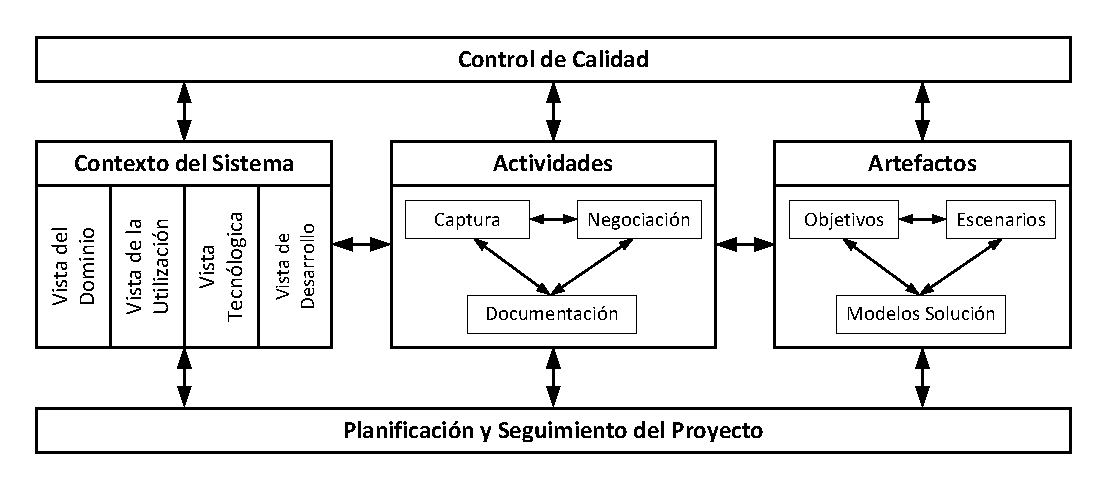
\includegraphics[width=11.5cm,keepaspectratio=true]{images/introduction/procesoIr00.eps}}
	}
    \only<2>{
	\rput[lt](0,-0.5){
	   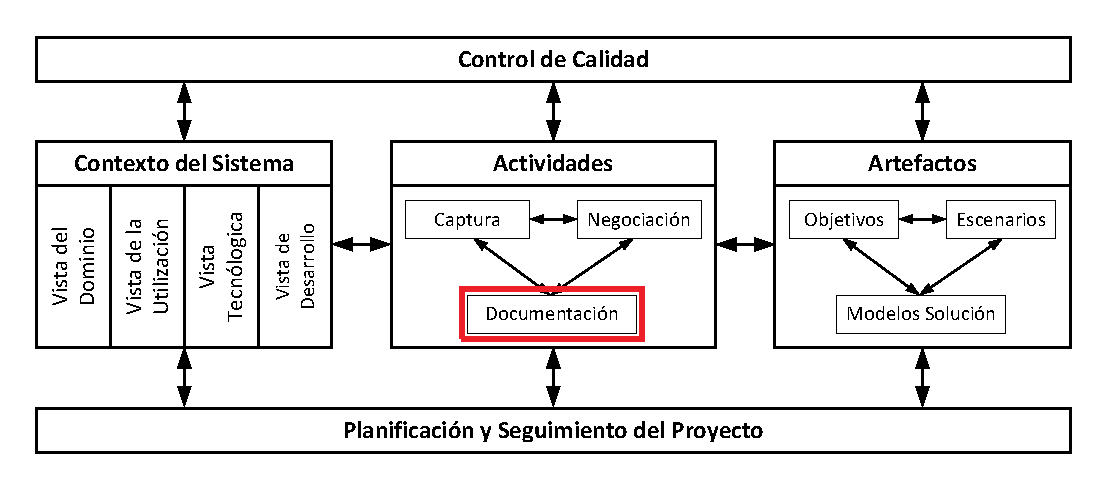
\includegraphics[width=11.5cm,keepaspectratio=true]{images/introduction/procesoIr01.eps}}
	}
    \only<3>{
	\rput[lt](0,-0.5){
	   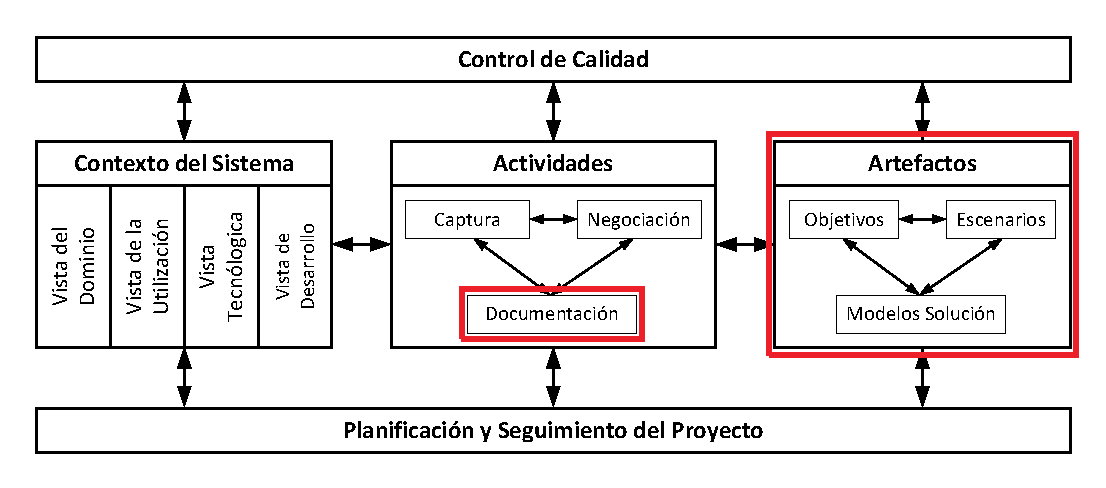
\includegraphics[width=11.5cm,keepaspectratio=true]{images/introduction/procesoIr02.eps}}
	}
\end{frame}

\subsection{Requisitos No Funcionales}

\begin{frame}[c]
    \frametitle{Requisitos No Funcionales}
    \begin{block}{Requisito No Funcional~\cite{chung:1999}}
        Un \alert{Requisito No Funcional} de un sistema sw es un requisito que no indica qué debe hacer el sistema, sino cómo debe hacerlo.
    \end{block}
\end{frame}

\subsection{Características de los Requisitos No Funcionales}

\begin{frame}[c]
    \frametitle{Características Requisitos No Funcionales}
    \begin{enumerate}[<+->]
        \item Suelen aplicarse al sistema como un todo, tienen influencia global.
        \item Aparecen recurrentemente en aplicaciones de diferente dominio.
        \item Su no satisfacción puede significar el fracaso del proyecto.
        %% Ejemplo: Incumplir una ley, no ser capaz de filtrar trolls
        \item Se materializan en requisitos funcionales frecuentemente.
        \item Pueden ser complejos y costosos de verificar.
        \item A pesar de su coste, podrían no utilizarse nunca.
        \item Suelen presentar conflictos entre ellos.
    \end{enumerate}
\end{frame}

\section{ISO 25010}

\begin{frame}[c]
    \frametitle{ISO 25010 - Calidad de un Producto Sw}
    \begin{center}
        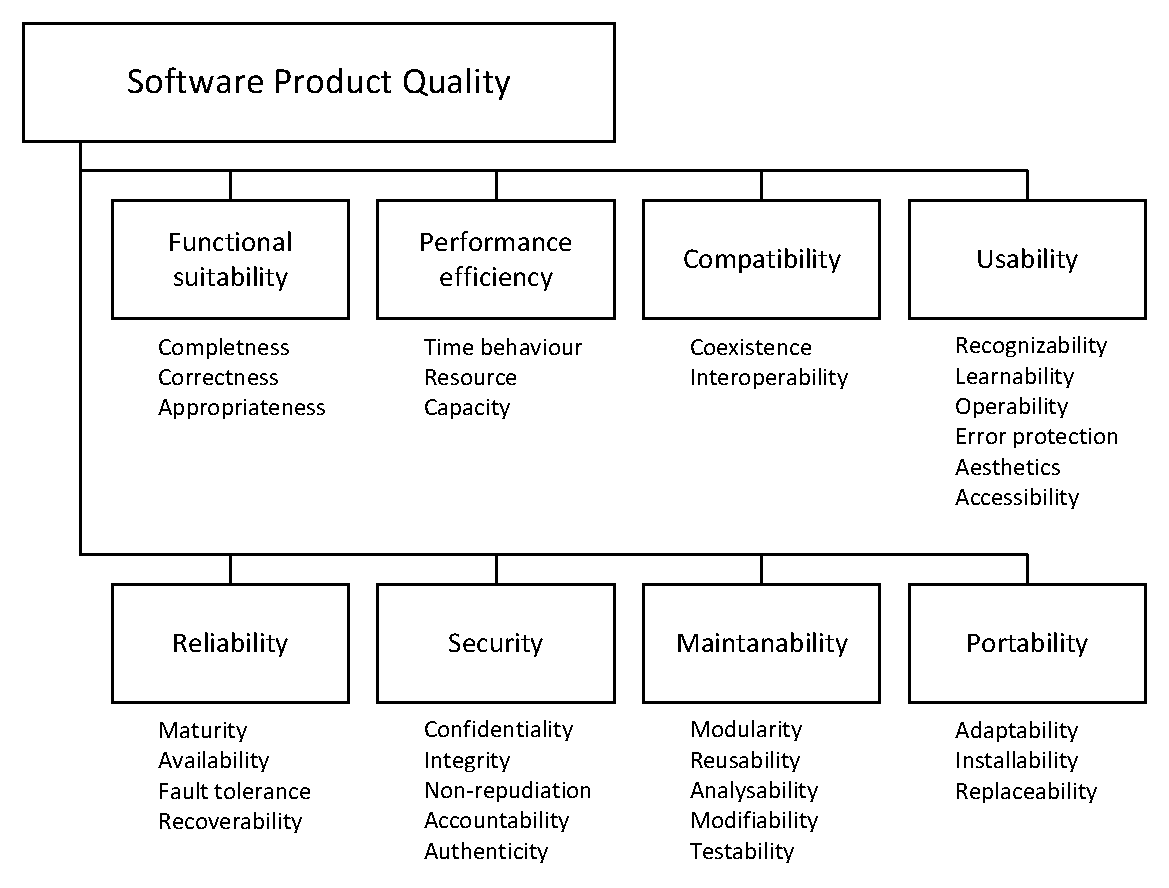
\includegraphics[width=0.85\linewidth]{images/iso25010/iso25010.eps}
    \end{center}
\end{frame}

\section{Sistemas Software Confiables}

\subsection{Sistemas Sociotécnicos}

\begin{frame}[c]
    \frametitle{Sistemas Sociotécnicos}
    \begin{block}{Sistemas Sociotécnicos}
        Un \emph{sistema sociotécnico} es un sistema empresarial diseñado para ayudar a conseguir un objetivo estratégico.
    \end{block}
    \begin{center}
        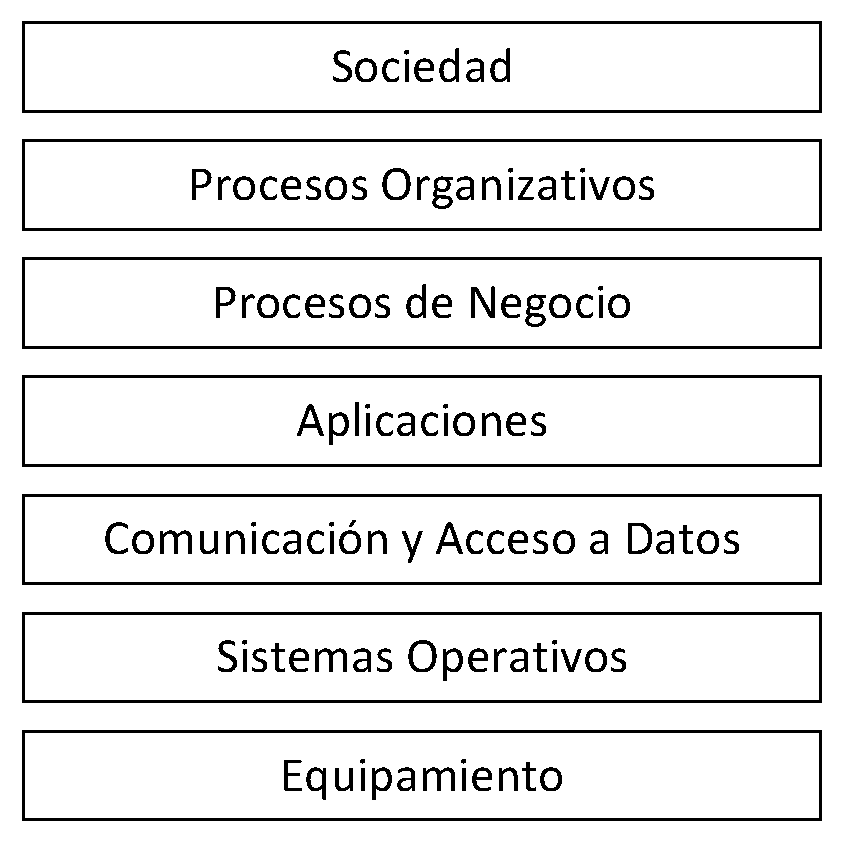
\includegraphics[width=0.40\linewidth]{images/sociotecnicos/layers.eps}
    \end{center}
\end{frame}

\subsection{Sistemas Software Confiables}

\begin{frame}[c]
    \frametitle{Sistemas Confiables}
    \begin{block}{Sistema Confiable (\emph{Dependeable System})}
        Un sistema se dice confiable cuando podemos tener cierta seguridad de que operará correctamente cuando lo necesitemos, no produciéndonos ni daños ni perjuicios. \uncover<2->{Un sistema confiable destaca por satisfacer cuatro requisitos no funcionales claves: (1) \emph{availability}; (2) \emph{reliability}; (3) \emph{safety}; y (4) \emph{security}.}
    \end{block}
\end{frame}

\begin{frame}[c]
    \frametitle{Sistemas Confiables}
    \begin{center}
        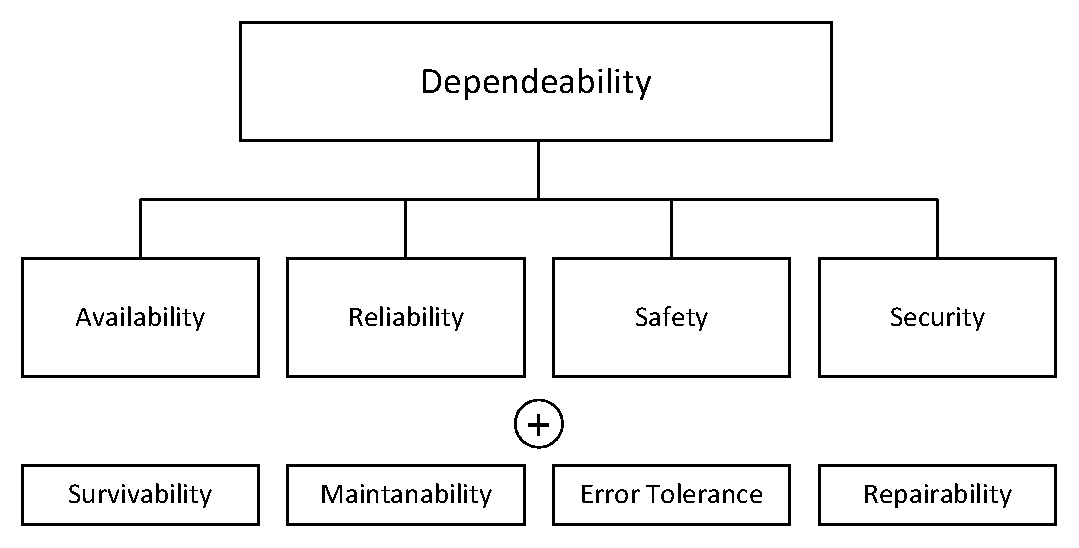
\includegraphics[width=\linewidth]{images/sociotecnicos/dependeability.eps}
    \end{center}
\end{frame}

\section{Modelado y Especificación de Requisitos de Seguridad}

\subsection{Introducción}

\begin{frame}[c]
    \frametitle{Seguridad de un Sistema Software~\cite{sommerville:2010}}
    \begin{block}{Seguridad de un Sistema Software}
        Capacidad de un sistema software de protegerse de ataques externos, los cuales pueden ser accidentales o deliberados, así como de resistirlos en caso de que se produzcan.
    \end{block}
    \uncover<2->{
        \begin{center}
            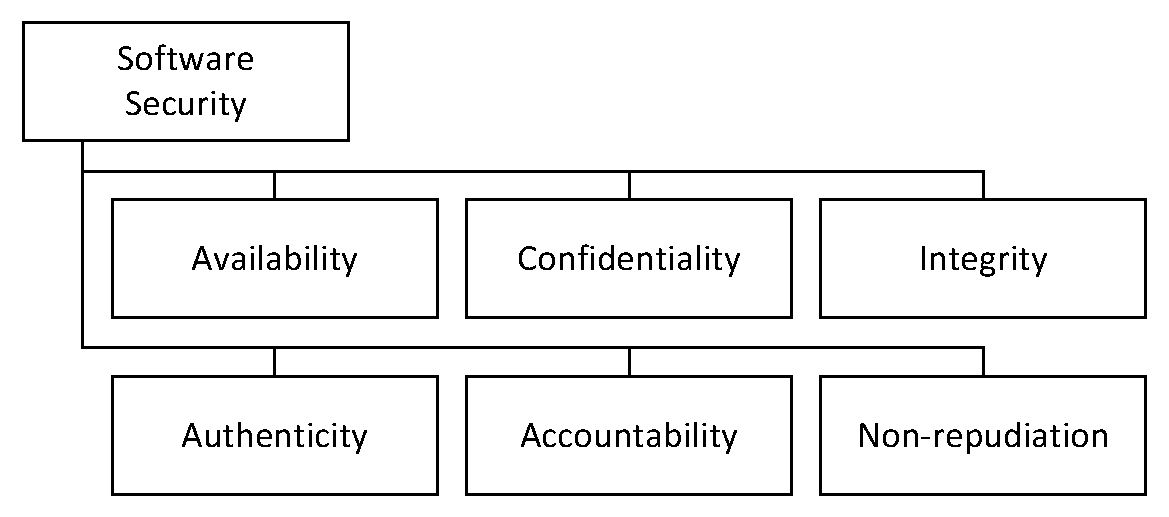
\includegraphics[width=0.85\linewidth,keepaspectratio=true]{images/security/decomposition.eps}
        \end{center}
	}
\end{frame}

\subsection{Terminología}

\begin{frame}[c]
    \frametitle{Terminología sobre Seguridad Software}
    \begin{description}[<+->]
        \item[Activo] Elemento (físico o lógico) de un sistema sw que posee cierto valor y por tanto debe protegerse de posibles ataques.
        %% Presidente del Gobierno
        \item[Amenazas] Evento que, de materializarse, causaría un daño o perjuicio al sistema.
        %% Muerte del presidente
        \item[Exposición] Perjuicio o daño que sufriría un sistema sw cuando se materializa una amenaza.
        %% Inestabilidad política, desplome económico del país
        \item[Vulnerabilidad] Debilidad de un sistema sw que puede explotarse para materializar una amenaza.
        %% Actos públicos
        \item[Ataque] Método concreto para materializar una amenaza a través de una vulnerabilidad.
        %% Utilizar un francotirador para asesinar al presidente mientras se desplaza por la calle a un acto público
        \item[Medida de Control] Decisión adoptada para reducir la vulnerabilidad de un sistema o para mitigar un ataque.
        %% Utilizar policías para controlar las ventanas y evitar la presencia de francotiradores
        \item[Premisa de Confianza] Hipótesis que ha de ser verdad para que la medida de control sea efectiva.
        %% Sólo puede haber francotiradores en las ventanas
        %% Los policías son de confianza
        \item[Contraargumento] Argumento que invalidaría la premisa de confianza.
        %% Se puede disparar desde ventanas cerradas.
        %% Hay policías están comprados por los asesinos
    \end{description}
\end{frame}

\subsection{Proceso de Ingeniería de Requisitos de Seguridad}

\begin{frame}[c]
    \frametitle{Proceso de Ingeniería de Requisitos de Seguridad}
    \begin{center}	
        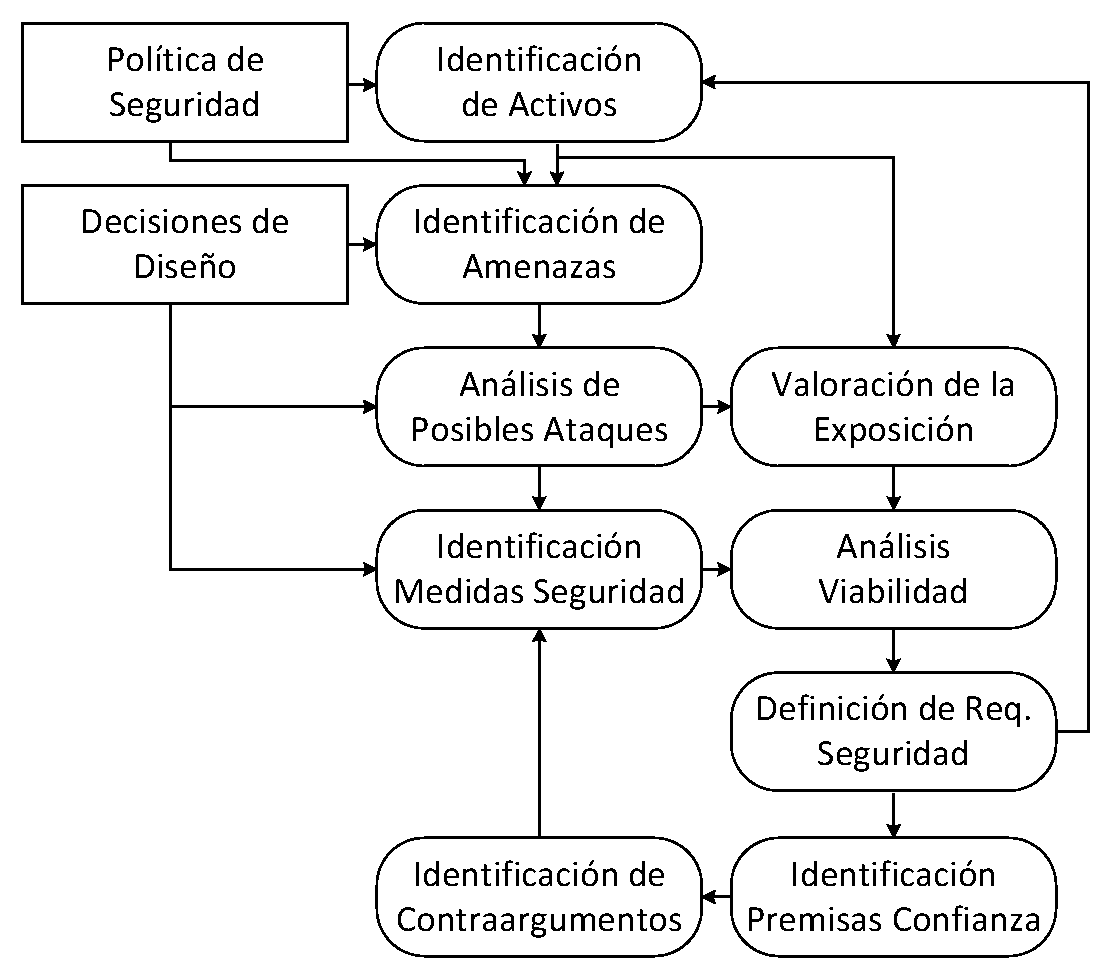
\includegraphics[width=0.65\linewidth,keepaspectratio=true]{images/security/sreProcess.eps}
    \end{center}
\end{frame}

\subsection{Tipos de Amenazas}

\begin{frame}[c]
    \frametitle{Modelo STRIPE de Amenazas}
    \begin{description}[<+->]
        \item[Spoofing] Suplantación fraudulenta de un tercero.
        \item[Tampering] Modificación no autorizada de datos.
        \item[Repudiation] Realización de acciones que impidan rastrear otras operaciones.
        \item[Information Disclosure] Acceso a información no autorizada.
        \item[Denial of Service] Impedir el acceso o utilización a usuarios legítimos.
        \item[Elevation of Privilege] Adquirir un rol que permita ejecutar acciones para los que no se posee permiso.
    \end{description}
\end{frame}

\subsection{Tipos de Medida de Control}

\begin{frame}[c]
    \frametitle{Técnicas Generales de Control de la Seguridad}
    \begin{enumerate}[<+->]
        \item Evitar o reducir el riesgo.
        %% Evitar accesos no autorizados
        \item Detección y neutralización de ataques.
        %% Detectar un borrado masivo de datos
        \item Limitación de la exposición y capacidad de recuperación.
        %% Mantener un registro de las operaciones realizadas y como neutralizarlas.
    \end{enumerate}
\end{frame}

%
%\begin{frame}[c]
%    \frametitle{Sistemas de Protección}
%    \begin{center}	
%        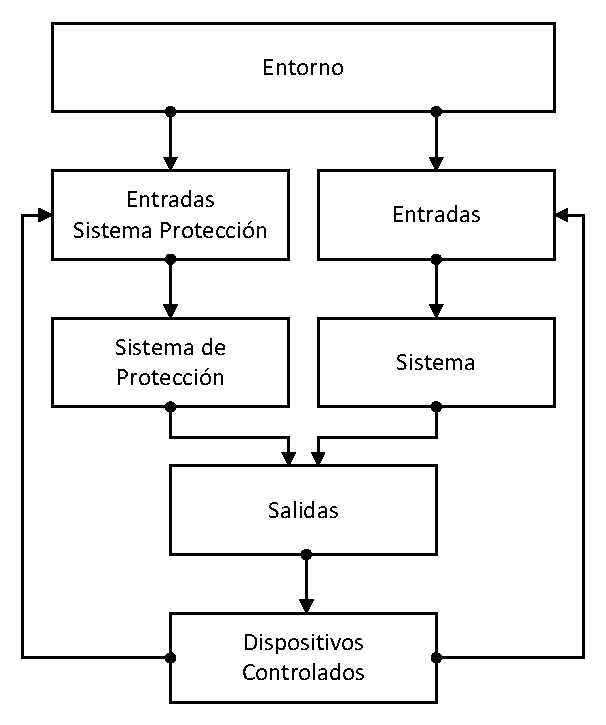
\includegraphics[width=0.50\linewidth,keepaspectratio=true]{images/security/sistemaProteccion.eps}
%    \end{center}
%\end{frame}

%\subsection[Casos de Mal Uso]{Casos de Mal Uso}
%
%\begin{frame}[c]
%    \frametitle{Casos de Mal Uso - Elementos}
%    \begin{block}{Actor de mal uso (\emph{Misuser})~\cite{Sindre2005}}
%        Actor(persona o sistema) que, de forma deliberada o no deliberada, inicia un caso de mal uso.
%    \end{block}
%    \uncover<2->{
%    \begin{block}{Caso de Mal Uso (\emph{Misuse Case})~\cite{Sindre2005}}
%        Escenario, incluyendo variaciones y extensiones, ejecutado por un actor de mal uso, que, si se ejecuta con éxito, constituye una amenaza para la seguridad del sistema.
%    \end{block}
%    }
%\end{frame}
%
%\begin{frame}[c]
%    \frametitle{Casos de Mal Uso - Relaciones}
%    \begin{block}{Amenaza (\emph{theaten})~\cite{Sindre2005}}
%        Relación entre un caso de mal uso y un caso de uso que indica que el el caso de mal uso utiliza o se basa en el caso de uso para ejecutar un ataque.
%    \end{block}
%    \uncover<2->{
%       \begin{block}{Mitiga (\emph{Mitigate})~\cite{Sindre2005}}
%            Relación entre un caso de uso y un caso de mal uso que indica que el caso de uso se utiliza para evitar o mitigar el daño o perjuicio causado por un caso de mal uso.
%       \end{block}
%    }
%\end{frame}
%
%\begin{frame}[c]
%    \frametitle{Casos de Mal Uso - Notación}
%    \begin{center}	
%        \includegraphics[width=\linewidth,keepaspectratio=true]{images/security/misusecase.eps}
%    \end{center}
%\end{frame}

\subsection{Directrices para la Gestión de la Seguridad}

\begin{frame}[c]
	\frametitle{Redundancia y Diversidad}
	\begin{block}{Redundancia}
		La \emph{redundancia} consiste en añadir recursos adicionales a un sistema de forma que puedan ser utilizados en caso de
		que fallen sus elementos principales.
	\end{block}
	\uncover<2->{
		\begin{block}{Diversidad}
			La \emph{diversidad} consiste en hacer que los recursos adicionales sean diferentes a los principales, de manera que se evite que un mismo fallo afecte a todos.
		\end{block}
	}
\end{frame}

\begin{frame}[c]
    \frametitle{Directrices para Garantizar la Seguridad Sw}
    \begin{enumerate}[<+->]
        \item Basar el proceso de gestión de la seguridad en la política de seguridad de la organización.
        \item Evitar los \emph{talones de Aquiles}.
        \item Fallar de forma segura.
        \item Balancear seguridad y usabilidad.
        \item Registrar las acciones de los usuarios.
        \item Utilizar redundancia y diversidad para reducir riesgos.
        \item Validar todas las entradas.
        \item Parcelar los activos.
        \item Gestionar y monitorizar el despliegue.
        \item Diseñar mecanismos de recuperación.
    \end{enumerate}
\end{frame}

%\begin{frame}[c]
%    \frametitle{Gestión y Monitorización del Despliegue}
%    \begin{enumerate}[<+->]
%        \item Incluir soporte para visualizar y analizar configuraciones.
%        \item Centralizar la gestión de la configuración de la aplicación.
%        \item Reducir los privilegios por defecto.
%        \item Proporcionar mecanismos simples para solucionar problemas de seguridad.
%    \end{enumerate}
%\end{frame}

%\section[Influencias entre Requisitos No Funcionales]{Modelado y Análisis de Influencias entre Requisitos No Funcionales}
%
%\subsection{Influencias entre NFRs}
%
%%% To animate
%\begin{frame}[t]
%    \frametitle{Influencias entre NFRs}
%    \only<1>{
%	\rput[lt](0,0){
%	   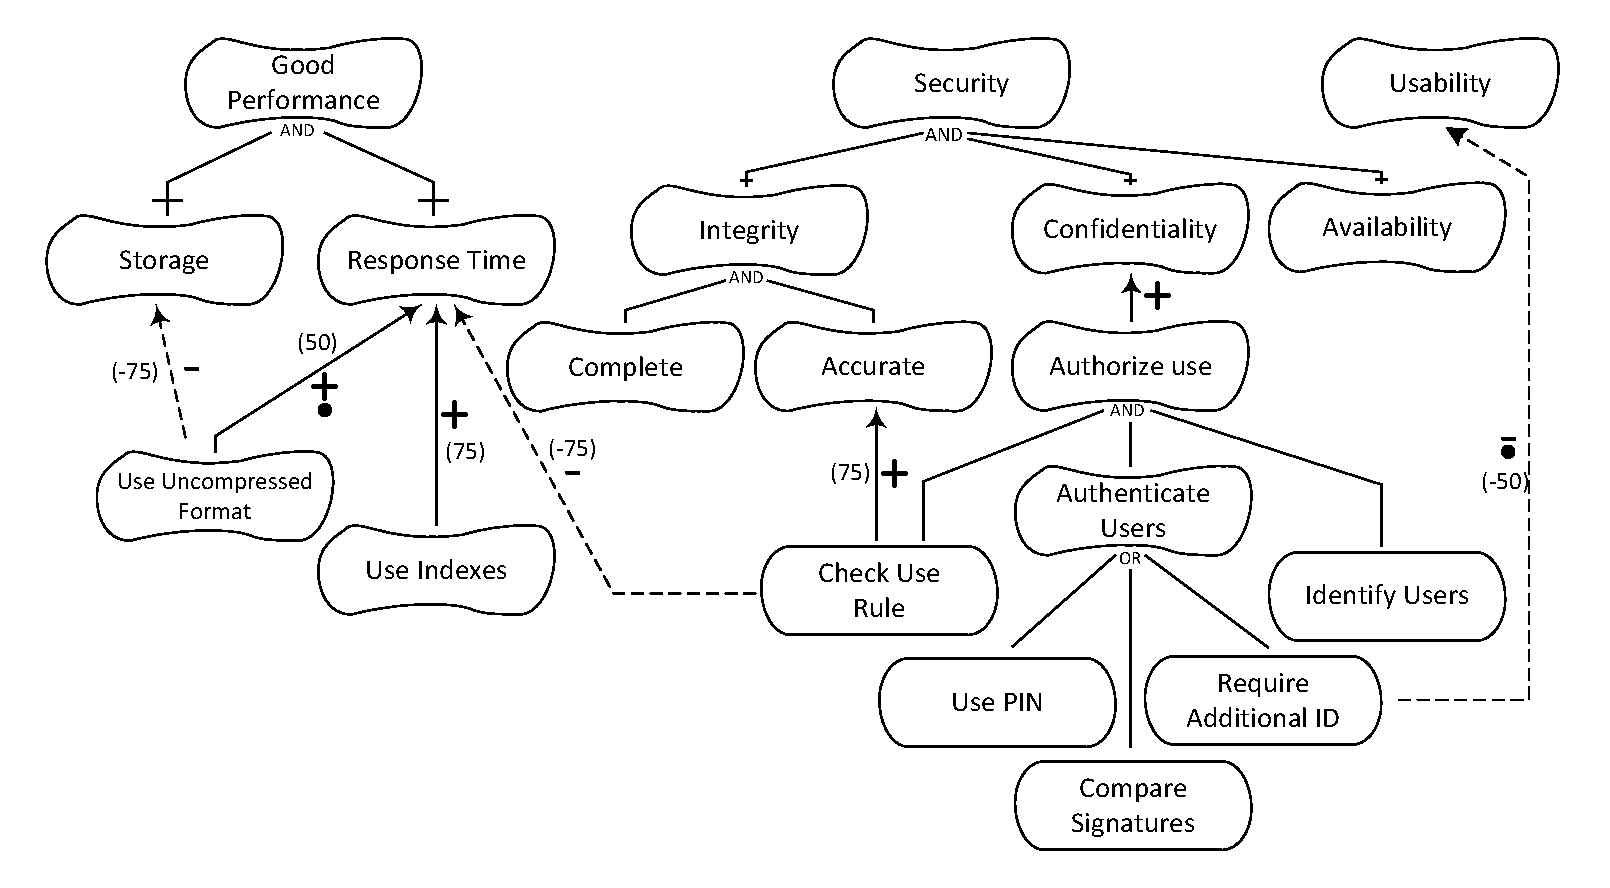
\includegraphics[width=12cm,keepaspectratio=true]{images/influences/nfrInfluences.eps}}
%	}
%\end{frame}
%
%\subsection{Evaluación de un Modelo de Objetivos}
%
%\begin{frame}[c]
%    \frametitle{Evaluación de Objetivos/Tareas Hoja}
%    \begin{block}{Regla de Evaluación de Objetivos/Tareas Hoja (Hao)}
%        \begin{center}
%    	   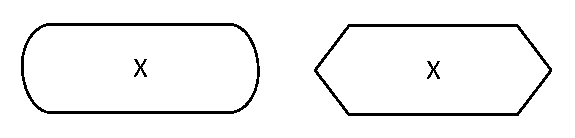
\includegraphics[width=0.5\linewidth,keepaspectratio=true]{images/influences/leafGoal.eps}
%        \end{center}
%        \begin{equation*}
%        V(X) =
%            \begin{cases}
%                100, \text{si\ } X \text{\ está seleccionado} \\
%                0, \text{otro caso}
%            \end{cases}
%        \end{equation*}
%        \ \\ \ \\
%    \end{block}
%\end{frame}
%
%\begin{frame}[c]
%    \frametitle{Evaluación de Relaciones AND}
%    \begin{block}{Regla de Evaluación de Relación AND (Hao)}
%        \begin{center}
%    	   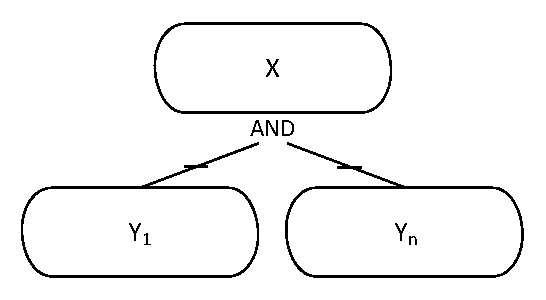
\includegraphics[width=0.4\linewidth,keepaspectratio=true]{images/influences/andRelationship.eps}
%        \end{center}
%        \begin{equation*}
%        V(X) = min_{i=1}^{n} V(Y_{i})
%        \end{equation*}
%        \ \\ \ \\
%    \end{block}
%\end{frame}
%
%\begin{frame}[c]
%    \frametitle{Evaluación de Relaciones OR}
%    \begin{block}{Regla de Evaluación de Relación OR (Hao)}
%        \begin{center}
%    	   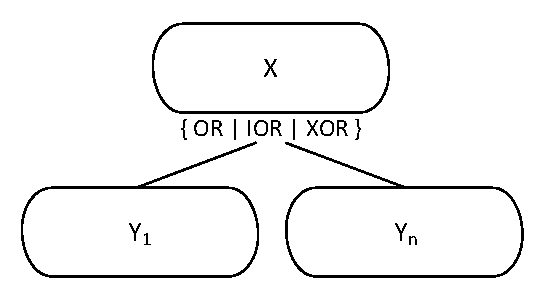
\includegraphics[width=0.4\linewidth,keepaspectratio=true]{images/influences/orRelationship.eps}
%        \end{center}
%        \begin{equation*}
%        V(X) = max_{i=1}^{n} V(Y_{i})
%        \end{equation*}
%        \ \\ \ \\
%    \end{block}
%\end{frame}
%
%\begin{frame}[c]
%    \frametitle{Evaluación de Contribuciones/Correlaciones}
%    \begin{block}{Regla de Evaluación de Contribuciones}
%        \begin{center}
%    	   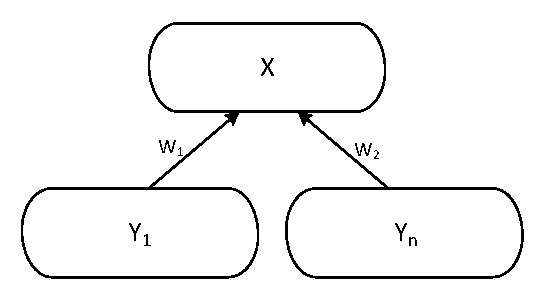
\includegraphics[width=0.4\linewidth,keepaspectratio=true]{images/influences/contributionRelationship.eps}
%        \end{center}
%        \begin{equation*}
%            V(X) = max(-100,min(100,\frac{\sum_{i=1}^{n} V(Y_{i})*W_{i}}{100}))
%        \end{equation*}
%        \ \\ \ \\
%    \end{block}
%\end{frame}
%
%\begin{frame}
%    \frametitle{Ejemplo 1: Índices y Verificación de Firmas}
%    \only<1>{
%	\rput[lt](0,0){
%	   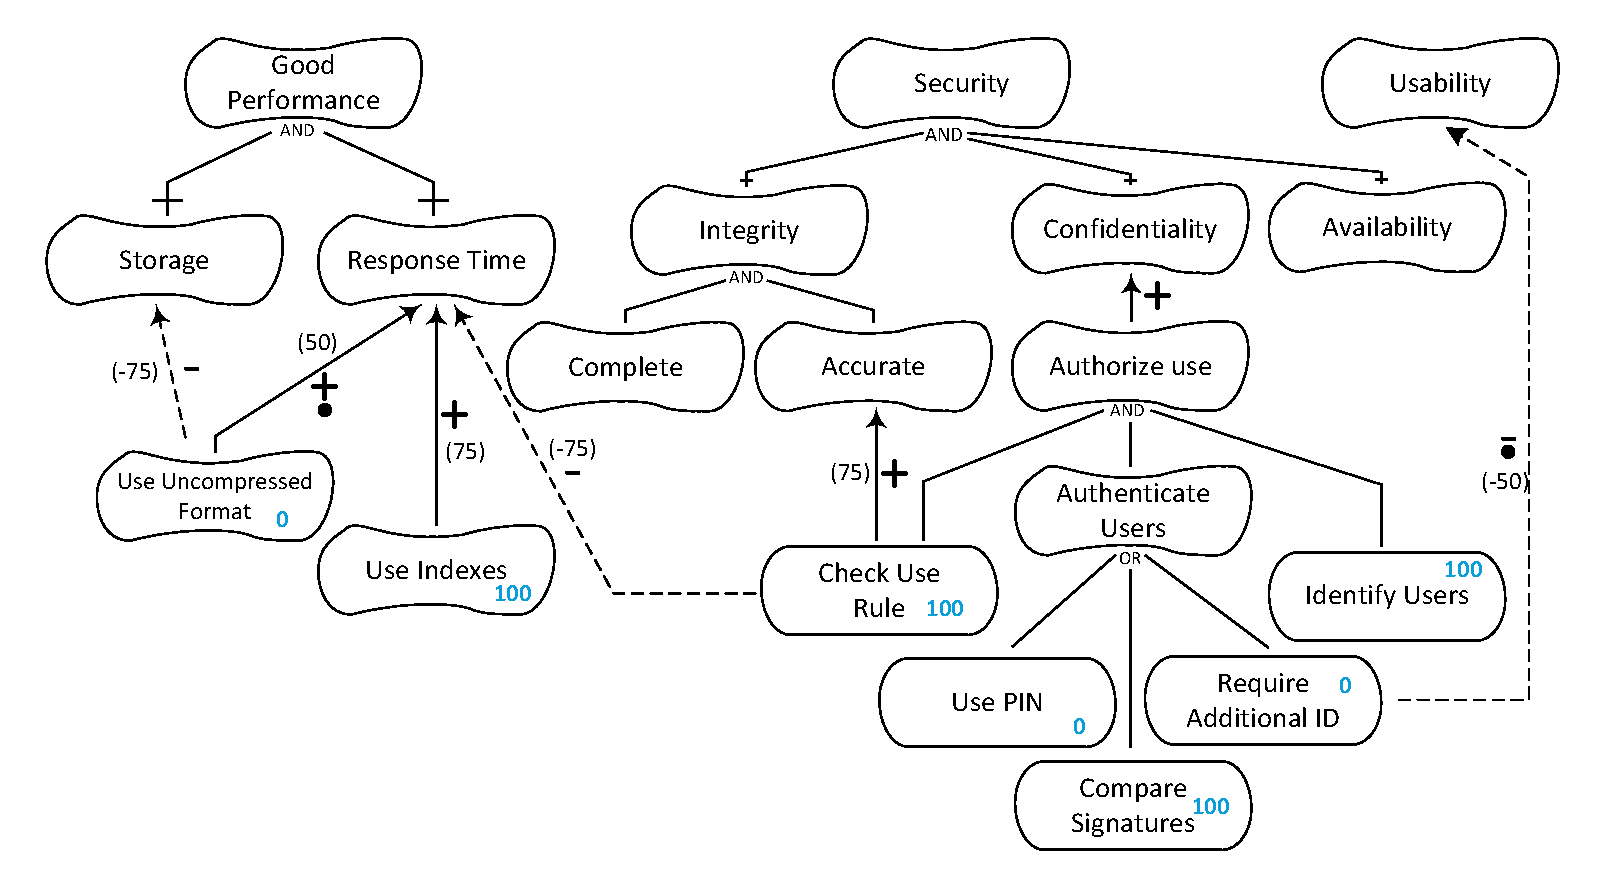
\includegraphics[width=11.5cm,keepaspectratio=true]{images/influences/example01_00.eps}}
%	}
%    \only<2>{
%	\rput[lt](0,0){
%	   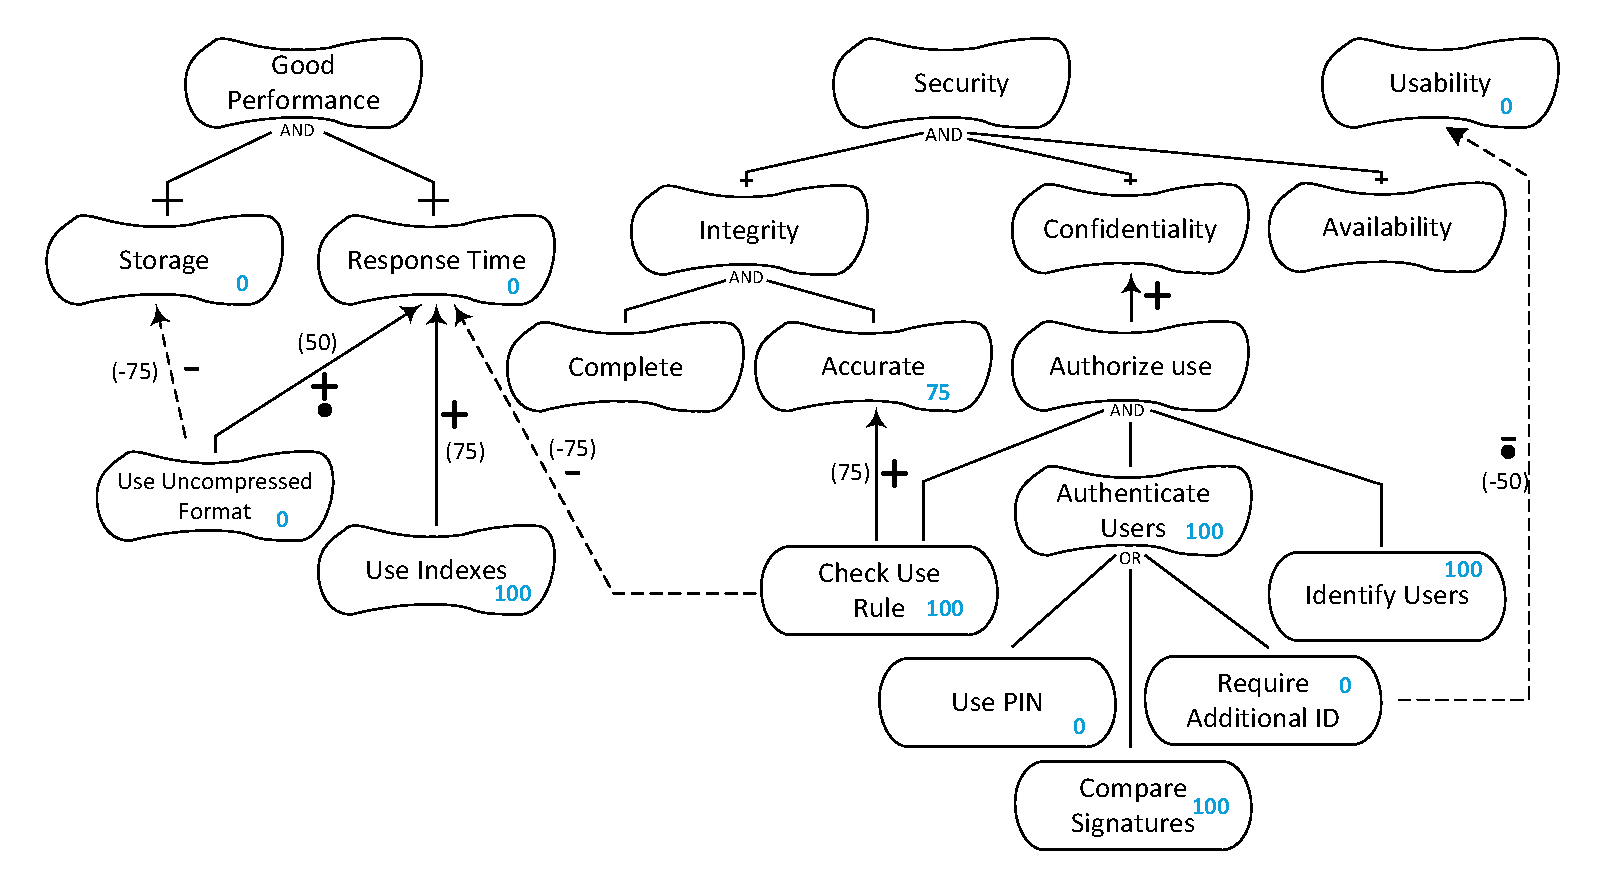
\includegraphics[width=11.5cm,keepaspectratio=true]{images/influences/example01_01.eps}}
%	}
%    \only<3>{
%	\rput[lt](0,0){
%	   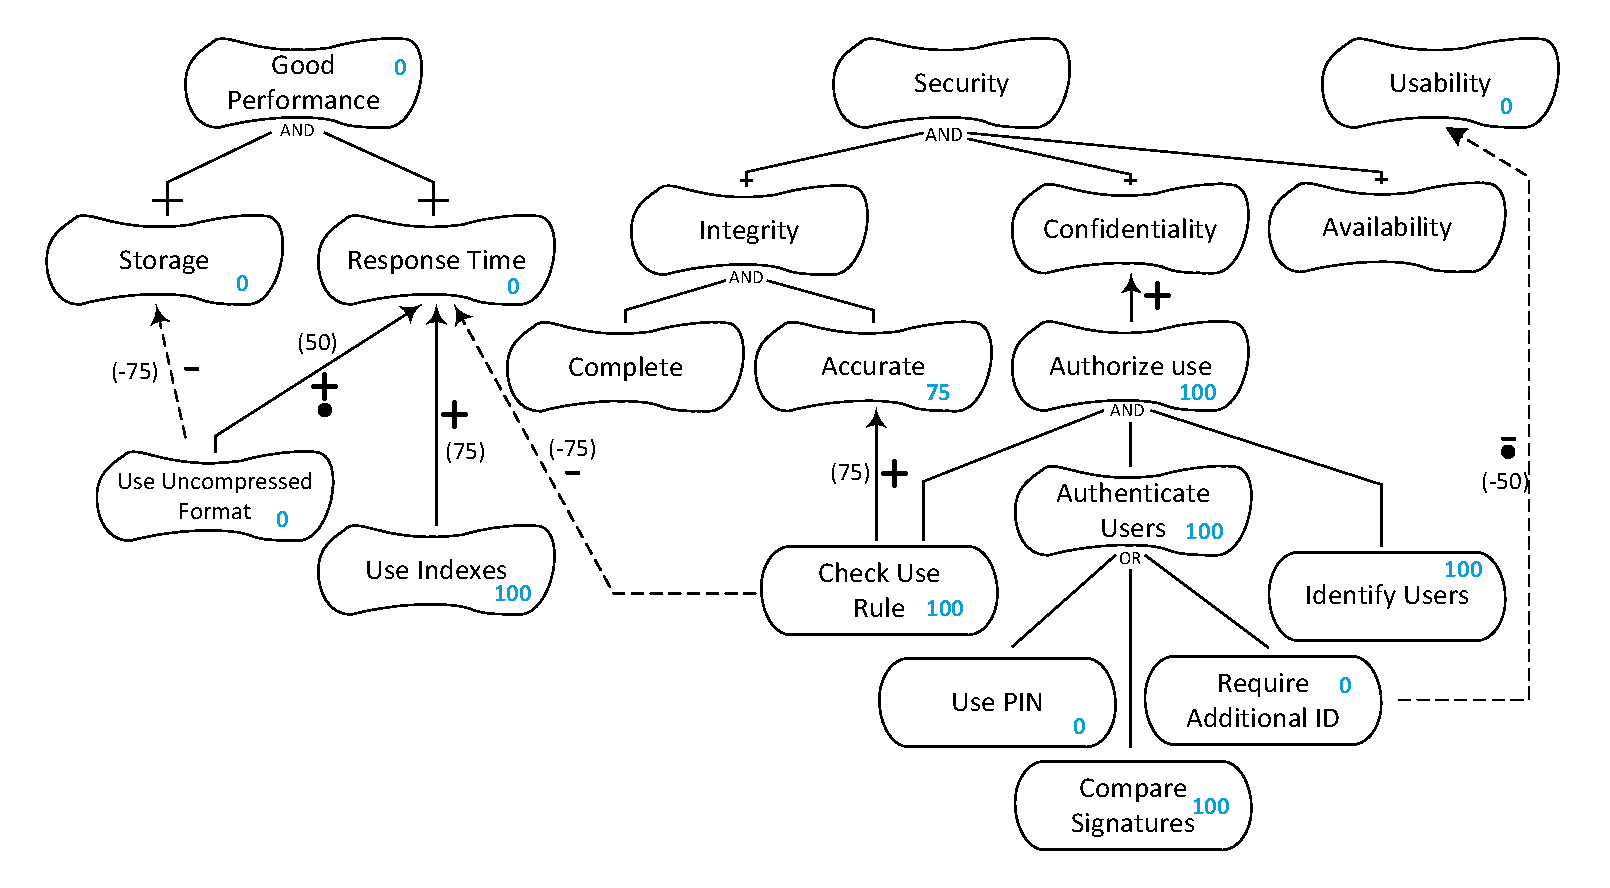
\includegraphics[width=11.5cm,keepaspectratio=true]{images/influences/example01_02.eps}}
%	}
%    \only<4>{
%	\rput[lt](0,0){
%	   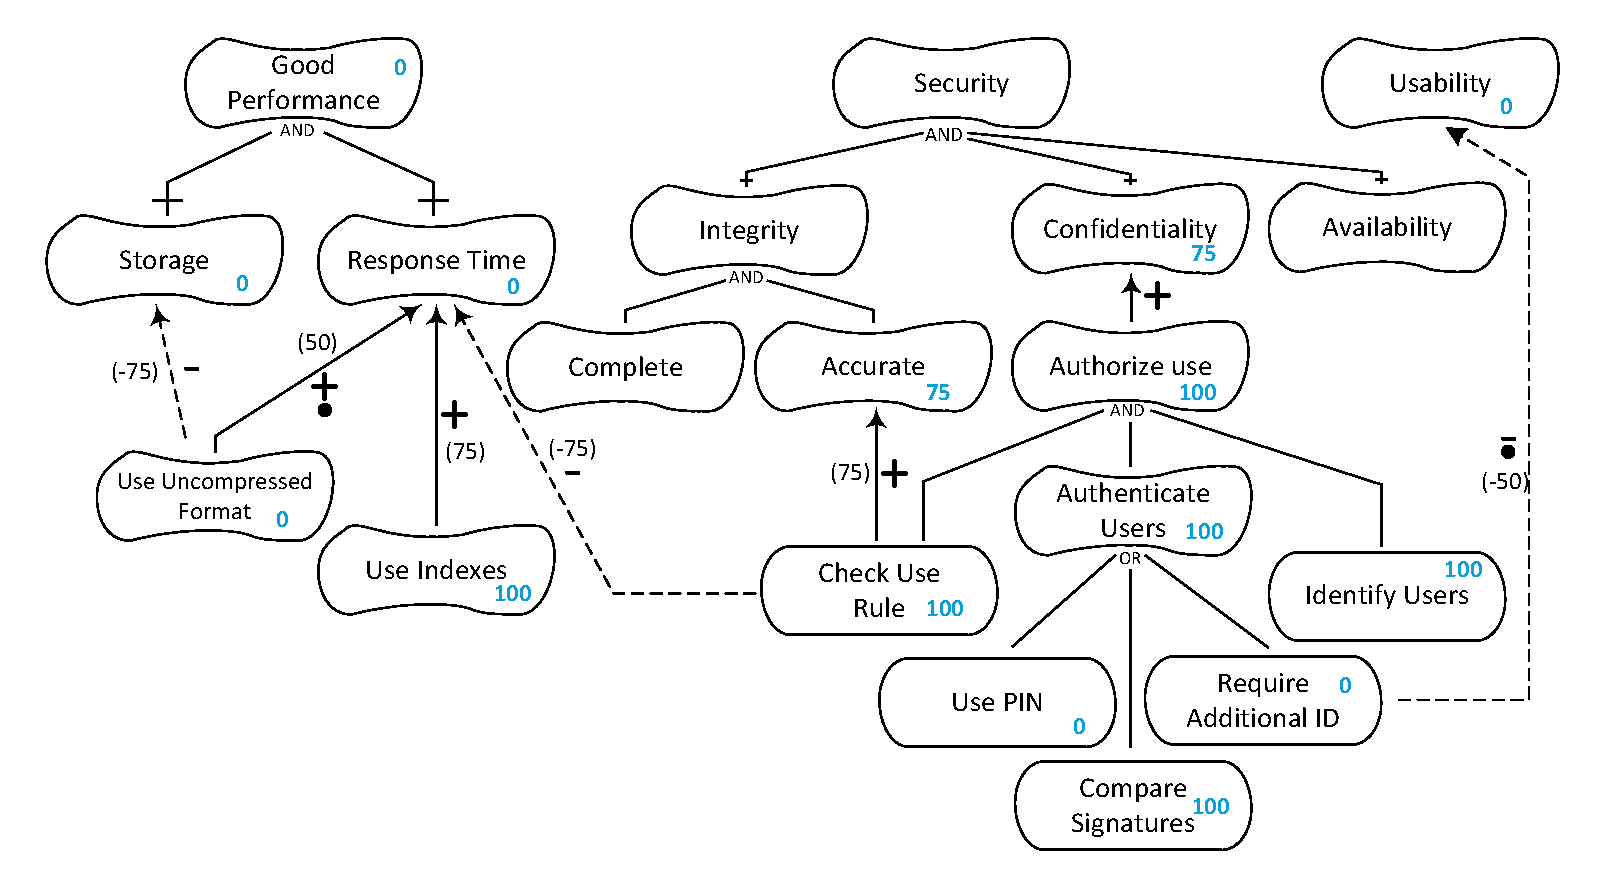
\includegraphics[width=11.5cm,keepaspectratio=true]{images/influences/example01_03.eps}}
%	}
%\end{frame}

\section{Negociación}

\subsection{Introducción}

\begin{frame}
    \frametitle{Proceso de Ingeniería de Requisitos}
    \only<1>{
	\rput[lt](0,-0.5){
	   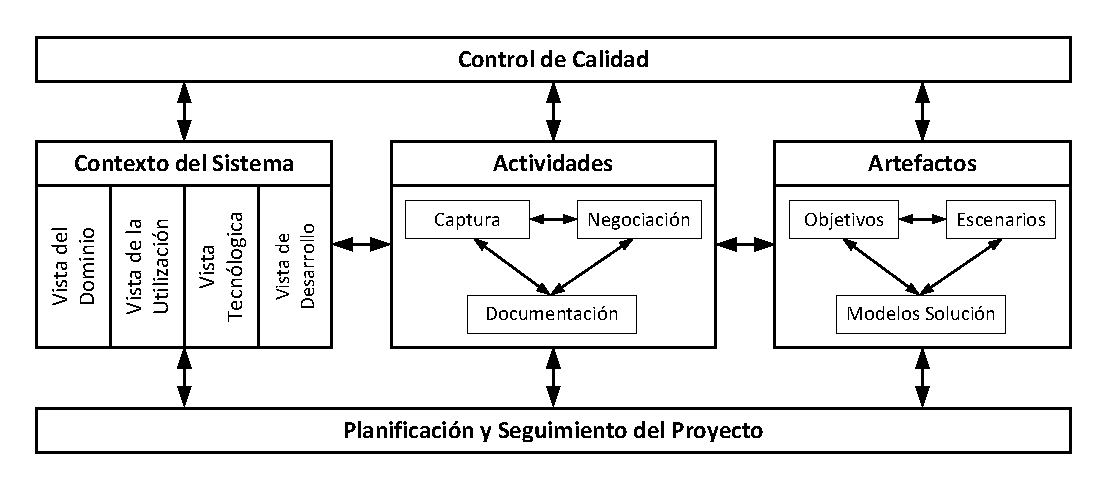
\includegraphics[width=11.5cm,keepaspectratio=true]{images/introduction/procesoIr00.eps}}
	}
    \only<2>{
	\rput[lt](0,-0.5){
	   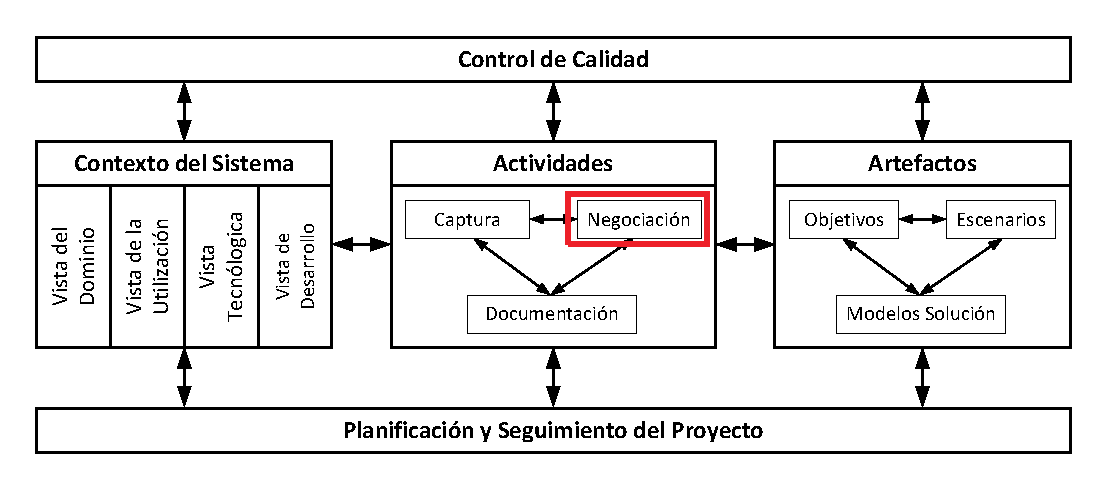
\includegraphics[width=11.5cm,keepaspectratio=true]{images/introduction/procesoIr03.eps}}
	}
\end{frame}

\subsection{Tipos de Conflictos}

\begin{frame}[c]
    \frametitle{Definición de Conflictos}
    \begin{block}{Conflicto en Ingeniería de Requisitos}
        Un conflicto en Ingeniería de Requisitos aparece cuando las necesidades y deseos de diferentes (grupos de) \emph{stakeholders} con respecto al sistema se contradicen, o si algunas necesidades y deseos no pueden ser tenidos en consideración.
    \end{block}
\end{frame}

\begin{frame}[c]
    \frametitle{Tipos de Conflictos}
    \begin{enumerate}
        %% Las recetas se muestran todas por orden alfabético.
        %% Las recetas se muestra por categorías y frecuencia de uso.
        \item Conflictos entre los datos recogidos.
        %% Buscar recetas de terceros en un amplio catálogo.
        %% Mantener y editar un recetario propio.
        \item Conflictos de intereses.
        %% Absolutamente necesario poder comunicarse entre usuarios.
        %% Totalmente imprescindible.
        \item Conflictos de valorización.
        %% Dos stakeholders tienen como objetivo no obtener un buen sistema, sino hacerse la puñeta mutuamente.
        \item Conflictos de relaciones interpersonales.
        %% Un stakeholder cuestiona, destruye o invalida trabajo de otro de categoría inferior con el simple
        %% objetivo de ejercer su autoridad.
        \item Conflictos estructurales.
    \end{enumerate}
\end{frame}

\subsection{Técnicas de Resolución}

\begin{frame}[c]
    \frametitle{Técnicas de Resolución de Conflictos}
    \begin{enumerate}
        \item Negociación (\emph{Win-Win}).
        \item Adoptar nuevas soluciones (\emph{Win-Win}).
        \item Decisión Externa.
    \end{enumerate}
\end{frame}

\subsection{Estrategias de Negociación}

\begin{frame}[c]
    \frametitle{Estrategias de Negociación}
    \begin{enumerate}
        \item Consider All Facts.
        \item Plus Minus Interesting.
    \end{enumerate}
\end{frame}

\begin{frame}[c]
	\frametitle{Estrategias \emph{Plus Minus Interesting}}
	\begin{enumerate}[<+->]
		\item Cada participante recibe una hoja con tres columnas o apartados, titulados \emph{Plus}, \emph{Minus}, e \emph{Interesting}.
		\item A continuación, cada participante escribe:
		\begin{itemize}[<+->]
			\item En la columna \emph{Plus}, aquellos elementos relacionados con el requisito en conflicto que son fundamentales para él.
			\item En la columna \emph{Minus}, aquellos elementos que no estaría dispuesto a admitir.		
			\item En la columna \emph{Interesting}, aquellos elementos que le agradan, pero a los que podría renunciar.		 
		\end{itemize}
		\item Finalmente, se examinan todas las hojas y se idean soluciones que traten de incluir todos los \emph{Plus}, excluir todos los \emph{Minus}, e incluir el máximo número de \emph{Interesting} posibles.
	\end{enumerate}
\end{frame}

\section{Sumario y Referencias}

\subsection{Sumario}

\begin{frame}[c]
    \frametitle{¿Qué Tengo que Saber de Todo Esto?}
    \begin{enumerate}[<+->]
        \item Comprender los rasgos diferenciadores de los \emph{requisitos no funcionales}.
        \item Comprender la terminología de la norma ISO 25010.
        \item Comprender el papel de los sistemas sw en los sistemas sociotécnicos.
        \item Comprender la importancia de los RNFs en los sistemas sociotécnicos.
        \item Ser capaz de analizar de la seguridad de un sistema sw.
        \item Ser capaz de especificar, a nivel básico, requisitos de seguridad para un sistema sw. 
        \item Saber especificar, modelar y analizar las influencias entre NFRs.
        \item Comprender los tipos de conflictos que pueden surgir entre requisitos.
        \item Ser capaz de aplicar la técnica \emph{Plus Minus Interesting}.
    \end{enumerate}
\end{frame}

\subsection{Referencias}

\begin{frame}
	\frametitle{Referencias}
	\bibliographystyle{apalike}
	\bibliography{ir}
\end{frame}

\end{document}
